\documentclass[11pt]{article}
\usepackage[utf8]{inputenc}
\usepackage[T1]{fontenc}
\usepackage{lmodern}
\usepackage[margin=2.5cm]{geometry}
\usepackage{amsmath,amssymb}
\usepackage{booktabs}
\usepackage{multirow}
\usepackage{graphicx}
\usepackage{xcolor}
\usepackage{tikz}
\usetikzlibrary{arrows.meta,positioning}
\usepackage[numbers,sort&compress]{natbib}
\usepackage[hidelinks]{hyperref}
\usepackage{microtype}

% незаповнені місця — видно в PDF, щоб нічого не пропустити перед подачею
\newcommand{\TBD}[1]{\textcolor{red}{[TBD: #1]}}

\title{Explainable Detection of Anomalous Unit Prices in Public Procurement:\\
Unsupervised Screening Calibrated on Auditor Verdicts}
\author{Dmytro Babarytskyi \and Tetiana Bilova\\[4pt]
\small Department of Computer Modeling and Intelligent Technologies,\\
\small Kharkiv National University of Radio Electronics, Kharkiv, Ukraine\\
\small dmytro.babarytskyi@nure.ua (ORCID 0009-0009-3614-9601, corresponding author);
tetiana.bilova@nure.ua (ORCID 0000-0002-1085-7361)}
\date{}

\begin{document}
\maketitle

\begin{abstract}
Public e-procurement systems publish millions of purchased items with their unit prices, yet price
screening in audit practice still relies on manual comparison or on procedure-level ``red flags'' that
ignore what was actually bought and at what price. We present a two-stage method for detecting anomalous
unit prices at the level of individual procured items and explaining each decision to an auditor. The
first stage makes heterogeneous item records comparable --- by converting per-package prices into prices
per kilogram or litre, grouping items hierarchically by procurement classification code and unit, and
splitting large groups by the semantics of their free-text descriptions --- and then screens each group
with robust statistical and density-based rules. The second stage is a gradient-boosting calibrator trained
on auditor verdicts that turns screening signals into the probability that an auditor would confirm the
anomaly; its decisions are explained per item with Shapley values expressed in auditor-readable terms.
We evaluate the method on 16{,}103 food items from the Ukrainian Prozorro system using a stratified,
design-weighted annotation of 400 items. We show that an annotator who sees the model's earlier decision
confirms its flags more often (anchoring), re-annotate the sample blind, and report agreement between the
two annotations ($\kappa = 0.82$). On blind labels, calibration raises the design-weighted average
precision from 0.49 to 0.81 (95\% bootstrap CI of the gain: 0.17--0.43) and F1 from 0.47 to 0.71,
outperforming statistical rules (3$\sigma$, Tukey) and unsupervised detectors (Isolation Forest, LOF,
ECOD). On injected errors the calibrator transfers to a held-out category without retraining, and
forcing gross extremes to be flagged restores recall of unit-scale errors at unchanged F1. Explanations
computed with 24 Monte-Carlo permutations deviate from a 2{,}000-permutation reference by about one risk
point and are faithful: removing the top feature lowers the risk by 88 points, a random one by 10.
The method is deployed in an open information system for auditors.
\end{abstract}

\noindent\textbf{Keywords:} public procurement; anomaly detection; price screening; explainable AI;
Shapley values; human-in-the-loop; audit analytics; decision support

%==============================================================================
\section{Introduction}

Public procurement accounts for a large share of government spending, and its digitalisation has made
transaction-level data openly available. The Ukrainian e-procurement system Prozorro alone registered
207 thousand procurements worth UAH~463 billion in a single quarter of 2025~\citep{prozorro2026q4}; each
procurement contains one or more items with a description, a classification code under the Common
Procurement Vocabulary (CPV, national version DK~021), a unit of measure, a quantity and --- in contracts or
in the expected value --- a price. This openness creates an opportunity for continuous, data-driven audit:
an auditor could, in principle, compare every purchased item with every comparable purchase.

In practice, item-level price screening is hard. Records that should be comparable are not: the same good
is bought per kilogram, per piece or per pack of unspecified weight, descriptions are free text, and a
single CPV code can cover goods whose prices differ by an order of magnitude. Data errors (a lot total
entered as a unit price, grams confused with kilograms) are as frequent as genuine over-pricing and are
equally relevant for an auditor, because they make published spending figures unreliable. Existing
automated risk indicators --- including those used by the Ukrainian State Audit Service~\citep{minfin2024indicators}
and the corruption risk indices of the procurement literature~\citep{fazekas2016objective,gti2024indicators}
--- operate at the level of procedures (single bidding, short tender periods, repeated winners) and largely
leave the price of what was bought unexamined.

Machine learning for procurement oversight has mostly been supervised on procedure-level outcomes, such as
sanctions, collusion cases or malfeasance reports~\citep{gallego2021preventing,huber2019screens,tas2024collusion},
or unsupervised over contract-level features~\citep{niessen2020ocds,torresberru2021mining}. Two obstacles
recur: labels are scarce and costly, and a flag without an explanation is hard for an auditor to act on.

This paper addresses item-level price screening as a decision-support problem with an auditor in the
loop. Our contributions are:
\begin{enumerate}
  \item \textbf{A comparability layer for item-level procurement prices}: pack-size parsing that converts
  per-piece prices into prices per kilogram or litre, hierarchical grouping by unit and CPV code with
  bottom-up aggregation of small groups, and semantic splitting of large groups by their descriptions.
  \item \textbf{A two-stage detector}: unsupervised screening within comparable groups (Tukey extremes,
  robust $z$-scores, DBSCAN in a joint price--quantity--season space) followed by a calibrator trained on
  auditor verdicts that outputs the probability of confirmation. Calibrator features are product-agnostic,
  so the model can be applied to categories it was not trained on.
  \item \textbf{Item-level explanations} with Monte-Carlo Shapley values over auditor-readable features,
  with an evaluation of their accuracy, stability and fidelity.
  \item \textbf{An evaluation protocol for label-scarce audit settings}: stratified annotation with
  Horvitz--Thompson weighting, a blind re-annotation that exposes and removes anchoring on the model's
  output, and a synthetic benchmark of error types typical of procurement data.
\end{enumerate}
The method is implemented in an information system that synchronises Prozorro data, runs the detector on
auditor-defined selections, and records verdicts with four-eyes approval; verdicts in turn retrain the
calibrator.

%==============================================================================
\section{Related work}

\paragraph{Risk indicators in public procurement.} Corruption risk research has developed composite
indices from procedure-level red flags~\citep{fazekas2016objective,gti2024indicators}. Their predictive
value is contested: red flags that are known in advance can be gamed, and the most scrutinised indicators
may be the least informative~\citep{decarolis2022redflags}. Ukrainian practice combines official automatic
indicators~\citep{minfin2024indicators} with civil-society tools such as DOZORRO, whose machine-learning
component scores procedures for likely violations~\citep{tiu2018dozorro}. None of these targets the unit
price of the purchased item.

\paragraph{Machine learning for procurement oversight.} Supervised models predict malfeasance from
procedure and municipality characteristics~\citep{gallego2021preventing}, detect bid rigging from
statistical screens of bid distributions~\citep{huber2019screens,tas2024collusion}, or predict corruption
indices~\citep{rabuzin2019prediction}. Unsupervised approaches apply clustering and outlier detection to
contract features~\citep{niessen2020ocds,torresberru2021mining,herreros2025purchase}. These works typically
treat a contract or lot as the unit of analysis; item descriptions and units of measure, which determine
whether two prices are comparable at all, receive little attention.

\paragraph{Unsupervised anomaly detection.} Robust univariate rules (Tukey fences~\citep{tukey1977eda},
the modified $z$-score~\citep{iglewicz1993outliers}) remain strong baselines for one-dimensional price data.
Density- and isolation-based detectors --- DBSCAN~\citep{ester1996dbscan}, LOF~\citep{breunig2000lof},
Isolation Forest~\citep{liu2008iforest}, ECOD~\citep{li2023ecod} --- extend screening to several attributes;
see~\citep{chandola2009survey} for a survey. Their output is a score with no notion of what a domain
expert would consider worth investigating.

\paragraph{Explanations and the human in the loop.} Shapley values~\citep{shapley1953value} provide
additive feature attributions with axiomatic guarantees; they are estimated by permutation sampling
for arbitrary models~\citep{strumbelj2014explaining} or computed efficiently for trees~\citep{lundberg2017shap,lundberg2020trees}.
Large language models have recently been used as annotators in text-classification tasks~\citep{gilardi2023chatgpt};
we use one under a written protocol and verify it against a human subsample. Anchoring on a provided
reference~\citep{tversky1974judgment} is a known threat when annotators see model output, which motivates
our blind re-annotation.

%==============================================================================
\section{Data and problem setting}\label{sec:data}

Prozorro publishes procurement records through an open API~\citep{prozorroapi} following the Open
Contracting Data Standard~\citep{ocds}. We synchronise the change feed into a document store and normalise
it into a relational schema of tenders, lots, items, contracts, procuring entities and suppliers. For every
item we derive a unit price from, in order of preference, an item-level unit value, the contract, or the
expected value, and we convert the unit of measure to a base unit (kilogram, litre, piece, \ldots) using
UN/CEFACT codes.

\begin{table}[h]
\centering
\caption{Data synchronised from Prozorro (change feed of 10--24 September 2026). The reference period is
publication between 1 August and 30 September 2026.}
\label{tab:data}
\small
\begin{tabular}{lrrrr}
\toprule
CPV division & Tenders & Items & Items with price and quantity & \ldots{} in reference period \\
\midrule
15 Food, beverages & 18{,}824 & 33{,}527 & 16{,}117 & 16{,}103 \\
03 Agricultural products & 7{,}850 & 21{,}266 & 6{,}511 & 6{,}507 \\
\bottomrule
\end{tabular}
\end{table}
Unit prices of CPV~15 items come from contracts (66\%), item-level unit values (25\%) and expected values
(9\%). CPV~15 is used for annotation and calibrator training; CPV~03 is held out to test transfer.

The analysis unit is an item with a positive unit price and quantity. The auditor selects CPV codes, a
publication period and optionally units; the detector returns, for every item, a risk score in $[0,100]$,
a binary decision and an explanation. The reference selection used for annotation is CPV division~15
(food products) published from 1~August to 30~September~2026: 16{,}103 items, of which 15{,}450 fall into
groups large enough to be analysed.

%==============================================================================
\section{Method}\label{sec:method}

\begin{figure}[t]
\centering
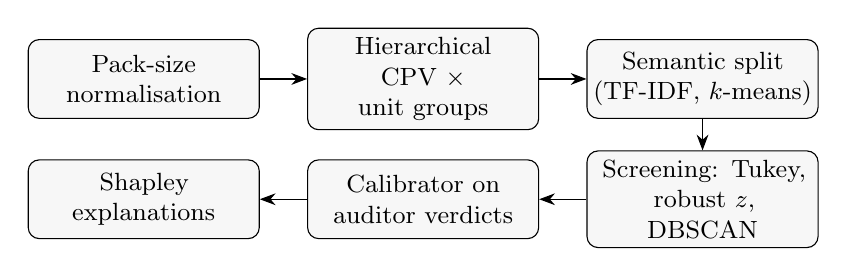
\begin{tikzpicture}[node distance=4mm and 6mm, every node/.style={font=\small},
  box/.style={draw, rounded corners, align=center, minimum height=10mm, text width=27mm, fill=gray!6},
  arr/.style={-{Stealth[length=2mm]}}]
\node[box] (pack) {Pack-size\\normalisation};
\node[box, right=of pack] (grp) {Hierarchical\\CPV $\times$ unit groups};
\node[box, right=of grp] (txt) {Semantic split\\(TF-IDF, $k$-means)};
\node[box, below=of txt] (scr) {Screening: Tukey,\\robust $z$, DBSCAN};
\node[box, left=of scr] (cal) {Calibrator on\\auditor verdicts};
\node[box, left=of cal] (shap) {Shapley\\explanations};
\draw[arr] (pack) -- (grp); \draw[arr] (grp) -- (txt); \draw[arr] (txt) -- (scr);
\draw[arr] (scr) -- (cal); \draw[arr] (cal) -- (shap);
\end{tikzpicture}
\caption{The two-stage pipeline: comparability layer (top), screening and calibration (bottom).}
\label{fig:pipeline}
\end{figure}

\subsection{Comparability layer}

\paragraph{Pack sizes.} Items bought per piece, pack, bottle or jar often state the net content in the
description (``sour cream 20\%, 350~g'', ``oil 5~l'', ``tea 20$\times$2~g''). A rule-based parser extracts the
content and converts the price to UAH per kilogram or litre; the quantity is converted accordingly.

\paragraph{Hierarchical groups.} Items are grouped by base unit and full eight-digit CPV code. Groups below
a minimum size ($n<10$) are merged upwards to the five-digit category and then to the four-digit class;
items that remain in groups smaller than the minimum are left unanalysed rather than compared with
dissimilar goods.

\paragraph{Semantic split.} A CPV code can still mix goods with very different prices (``dairy products''
covers yoghurt and hard cheese). Groups with at least 30 items are split by description: lemmatised
descriptions are vectorised with TF-IDF~\citep{salton1988weighting}, reduced with truncated SVD and
clustered with $k$-means, choosing $k\le 8$ by the silhouette coefficient~\citep{rousseeuw1987silhouettes};
the split is kept only if the silhouette exceeds 0.15 and every subgroup has at least five items.

\subsection{Unsupervised screening}

Within each group $g$ with log prices $\ell_i$:
\begin{enumerate}
\item \emph{Extremes}: $\ell_i$ outside $[Q_1-3\,\mathrm{IQR},\,Q_3+3\,\mathrm{IQR}]$; extremes are excluded
from the estimation of the group's centre and spread.
\item \emph{Robust $z$-score}: $z_i=(\ell_i-\tilde\ell_g)/\max(1.4826\,\mathrm{MAD}_g,\,0.15)$, where the floor
prevents ordinary market variation of about 15\% from being flagged in very homogeneous groups.
\item \emph{Density outliers}: DBSCAN~\citep{ester1996dbscan} in the PCA projection~\citep{jolliffe2016pca}
of standardised $[2\ell, \log q, \sin m, \cos m]$ (price weighted twice, quantity, cyclically encoded month),
with $\varepsilon$ chosen at the knee of the sorted $k$-distance curve~\citep{satopaa2011kneedle}.
\end{enumerate}
An item is flagged if it is an extreme, or $|z_i|\ge4$, or it is a density outlier with $|z_i|\ge3$: a
density outlier must be a \emph{price} outlier, not merely unusual in quantity or date.

\subsection{Calibration on auditor verdicts}

Screening finds deviations but cannot know which deviations an auditor considers worth investigating.
A gradient-boosting classifier~\citep{friedman2001gbm,ke2017lightgbm} (histogram-based, depth~3, 300
iterations, balanced class weights) maps 19 screening and context features to the probability that an
auditor confirms the item: the signed and absolute robust $z$, the log ratio to the group median, extreme
and density-outlier indicators, group size and spread, TF-IDF distance of the description to the group
centroid, an indicator of generic descriptions (``various food products''), pack conversion and a
``price-per-pack'' mismatch feature (how close the log ratio is to the log pack size), unit type, price
source, and log quantity. None of the features identifies a product, which is what allows transfer
across categories. The decision threshold is selected by cross-validation.

With few positive labels, an unconstrained tree ensemble can learn non-monotone relations from
idiosyncrasies of the sample --- in our first blind-trained model, a twelvefold over-priced item with a
converted pack size received a lower probability than moderate deviations. We therefore impose monotone
constraints: the predicted probability is non-decreasing in the absolute robust $z$-score and in the
extreme indicator. The constraint encodes domain knowledge that a larger deviation is never less
suspicious, other things equal; on the annotated sample it leaves ranking quality unchanged and lowers
precision at the selected threshold (Section~\ref{sec:results}).

The calibrator is retrained offline when enough new verdicts have accumulated (in our deployment we plan a
semi-annual to annual cycle), rather than continuously: verdicts given while the auditor sees the model's
output carry the anchoring bias described in Section~\ref{sec:res-labels}, and periodic retraining allows
the training set to be audited first.

\subsection{Explanations}

For an item $x$ the contribution of feature $j$ is its Shapley value with respect to background items
$z$ drawn from unflagged items of the same selection,
\begin{equation}
\phi_j(x)=\sum_{S\subseteq F\setminus\{j\}}\frac{|S|!\,(d-|S|-1)!}{d!}\left[f(x_{S\cup\{j\}},z_{\bar S\setminus\{j\}})-f(x_S,z_{\bar S})\right],
\end{equation}
estimated by Monte Carlo over random feature permutations~\citep{strumbelj2014explaining} (24
permutations per item in the deployed system). Contributions are reported in risk points and labelled in
the auditor's language (e.g.\ ``strength of deviation from the group median'', ``price resembles a
per-pack price'').

%==============================================================================
\section{Evaluation design}\label{sec:eval}

\paragraph{Stratified annotation.} True anomalies are rare, so a simple random sample would contain few
positives. We stratified the reference selection by the decision of the first system version (v1): the 50
highest-risk flagged items (\emph{top}), the remaining 577 flagged items (\emph{mid}) and 14{,}823 unflagged
analysed items (\emph{normal}); 50, 100 and 250 items were annotated respectively. Population metrics are
estimated with Horvitz--Thompson weights $w_h=N_h/n_h$~\citep{horvitz1952sampling}; confidence intervals use a
stratified bootstrap with 2{,}000 replicates~\citep{efron1993bootstrap}.

\paragraph{Annotation protocol.} An item is \emph{confirmed} if an auditor should examine its unit price:
a substantial deviation from comparable goods not explained by the description (as a guide, above
$\sim$2$\times$ or below $\sim$0.4$\times$ the typical price), a price that clearly refers to another unit
(pack, gram, whole lot), or another evident data error. Items whose description does not allow a judgement
are marked \emph{cannot judge} and excluded. Annotation was performed by a large language model (Claude,
Anthropic) under this written protocol; a human annotator re-labelled a subsample of 80 items
(Section~\ref{sec:res-labels}).

\paragraph{Anchoring and blind re-annotation.} In the first annotation round, annotation cards displayed
the v1 decision and risk score. Because this can anchor the annotator on the model's output, we
re-annotated all 400 items \emph{blind}: cards show only the item record and neutral reference prices
(median, 10th--90th percentile and eight random examples of items with the same CPV code and unit, drawn
directly from the database rather than from the pipeline's groups), in shuffled order. All results below use
the blind labels unless stated otherwise.

\paragraph{Calibrator evaluation.} The calibrator is evaluated with nested cross-validation: five outer
folds repeated five times; in each outer training set the decision threshold is chosen by an inner
five-fold cross-validation maximising design-weighted F1. Reported calibrator scores therefore come only
from models that have not seen the item and whose threshold was not tuned on it.

\paragraph{Baselines and alert budget.} We compare with 3$\sigma$ and Tukey rules on log prices within
CPV class $\times$ unit (an auditor without the system) and within the eight-digit code, and with
Isolation Forest, LOF and ECOD applied (i) to log prices within the pipeline's groups and (ii) to the 19
calibrator features without labels. Since unsupervised detectors have no natural threshold, we compare them
at an equal alert budget of 4\% of analysed items (the share flagged by v1) and by average precision (AP),
which does not depend on a threshold.

\paragraph{Synthetic errors.} Annotations measure what an annotator considers relevant; they cannot
measure recall for error types that are rare in a 400-item sample. We therefore inject errors with known
ground truth into 3\% of items, in equal shares of four types typical of procurement records:
\emph{moderate} price deviations ($\times2$, $\times3$, $\times0.4$, $\times0.5$), \emph{strong} deviations
($\times5$, $\times10$, $\times0.1$, $\times0.2$), \emph{unit-scale} errors ($\times1000$ or $\times0.001$,
grams vs.\ kilograms, kilograms vs.\ tonnes) and \emph{lot totals} entered as unit prices (price multiplied
by the quantity, for items with quantity $\ge5$). We repeat the injection with three seeds in CPV~15 and in
the held-out CPV~03 and apply the calibrators without retraining. Genuine anomalies already present in the
data are unlabelled and count as false positives, so precision is a lower bound; recall by error type is
exact.

%==============================================================================
\section{Results}\label{sec:results}

\subsection{Annotation agreement and anchoring}\label{sec:res-labels}

Of the 400 items, the blind annotation confirmed 54 and marked 9 as \emph{cannot judge}. Agreement between
the sighted and the blind annotation is high (Cohen's~\citep{cohen1960kappa} $\kappa=0.82$ on the 376 items
judged in both rounds; $\kappa=0.68$ including the \emph{cannot judge} class), but the disagreements are not
symmetric. Among items flagged by v1, the sighted annotation confirmed 14 that the blind annotation did not,
against 4 in the opposite direction; confirmation rates fell from 52\% to 42\% in the top stratum and from
37\% to 32\% in the mid stratum. Seeing the model's decision thus inflated agreement with the model ---
an anchoring effect that would bias any evaluation built on such labels.
A human annotator (not a professional auditor) labelled a subsample of 80 blind cards (30 confirmed and 50
not confirmed by the blind annotation, order shuffled, annotation hidden). On the 78 items both judged,
raw agreement was 82\% and $\kappa=0.64$. Disagreements were again asymmetric: the human flagged 12 items
the model did not, against 2 in the opposite direction. Most of the 12 are goods whose neutral reference
prices are not truly comparable --- vanilla sugar shown next to ordinary sugar, dry yeast next to fresh
yeast, whole-grain pasta, juice in 200~ml packs --- where the human followed the reference prices literally
and the model adjusted for the product. Comparability thus limits not only automatic screening but also
human judgement, which supports the emphasis of Section~\ref{sec:method} on the comparability layer.

\subsection{Detection quality}

\begin{table}[t]
\centering
\caption{Design-weighted quality on blind labels (reference selection, CPV 15). P, R, F1 at the method's
own threshold or at the 4\% alert budget; AP is threshold-free.}
\label{tab:labels}
\small
\begin{tabular}{lcccc}
\toprule
Method & P & R & F1 & AP \\
\midrule
3$\sigma$, CPV class $\times$ unit & 0.489 & 0.427 & 0.456 & 0.506 \\
Tukey (IQR), CPV class $\times$ unit & 0.274 & 0.645 & 0.384 & 0.455 \\
Tukey (IQR), CPV code $\times$ unit, 4\% budget & 0.331 & 0.623 & 0.432 & 0.449 \\
Isolation Forest in pipeline groups, 4\% & 0.413 & 0.711 & 0.522 & 0.395 \\
LOF in pipeline groups, 4\% & 0.219 & 0.715 & 0.336 & 0.176 \\
ECOD in pipeline groups, 4\% & 0.245 & 0.776 & 0.372 & 0.285 \\
Isolation Forest on calibrator features, 4\% & 0.150 & 0.405 & 0.219 & 0.153 \\
ECOD on calibrator features, 4\% & 0.171 & 0.492 & 0.254 & 0.176 \\
\midrule
v1 (screening only) & 0.339 & 0.780 & 0.473 & 0.493 \\
\quad + pack-size normalisation & 0.473 & 0.952 & 0.632 & 0.544 \\
\quad + finer semantic split (v2 screening) & 0.478 & 0.952 & 0.637 & 0.544 \\
v2 screening without CPV grouping & 0.405 & 0.423 & 0.414 & 0.382 \\
v2 screening without semantic split & 0.320 & 0.602 & 0.418 & 0.358 \\
\midrule
\textbf{v2: screening + monotone calibrator (nested CV)} & \textbf{0.637} & \textbf{0.796} & \textbf{0.708} & \textbf{0.808} \\
Hybrid: extremes always flagged + calibrator & 0.500 & 0.865 & 0.634 & 0.612 \\
\bottomrule
\end{tabular}
\end{table}

Table~\ref{tab:labels} summarises the results. Three findings stand out. First, comparability matters more
than the choice of detector: removing CPV grouping or the semantic split lowers AP of the screening stage
from 0.54 to 0.38 and 0.36, while pack-size normalisation alone raises F1 from 0.47 to 0.63. Second, generic
unsupervised detectors do not beat simple robust rules on this problem: within the same groups, Isolation
Forest, LOF and ECOD reach AP of 0.18--0.40, below the screening stage (0.54); applied to the 19 calibrator
features without labels they perform worst (AP 0.15--0.18), because those features are informative only
in combination with the auditor's notion of relevance. Third, calibration on verdicts is the largest single
improvement in ranking quality: AP rises from 0.49 (v1) to 0.81, with a stratified-bootstrap 95\%
interval of $[0.17, 0.43]$ for the gain and no replicate showing a loss. The gain in F1 at the selected
threshold (0.47 $\to$ 0.71) is less certain, $[-0.01, 0.44]$, because the threshold is chosen on few
positives in inner folds. An unconstrained calibrator reached a higher F1 (0.78) at the same AP; the
monotone constraint trades some precision for guaranteed behaviour on extreme deviations (see below).
Forcing every extreme to be flagged (hybrid) lowers AP to 0.61: annotators do not consider every extreme
price relevant, often because the good is not comparable with its group. On the sighted labels the
conclusions are unchanged (AP 0.47 $\to$ 0.75, F1 0.47 $\to$ 0.75).

\paragraph{Sensitivity to the annotator.} Substituting the human labels on the 80 verified items changes
the picture considerably: 63 instead of 54 items are confirmed, most of the additions are goods whose
reference prices are not comparable, and all methods lose quality (v1: AP 0.36; screening stage of v2:
AP 0.44). The calibrated model remains the best ranker (AP 0.48, F1 0.43), but its gain over v1 is no
longer significant (AP gain 95\% CI $[-0.04, 0.33]$). The benefit of calibration is therefore tied to a
consistent notion of relevance in the labels it is trained and evaluated on.

\subsection{Synthetic errors and transfer to another category}

\begin{table}[t]
\centering
\caption{Injected errors (3\% of items, three seeds; mean). Precision is a lower bound; R by type is
recall for moderate, strong, unit-scale and lot-total errors. Calibrators are trained on CPV~15 labels and
applied without retraining; CPV~03 is held out.}
\label{tab:synthetic}
\small
\setlength{\tabcolsep}{4pt}
\begin{tabular}{llccccccc}
\toprule
 & Method & F1 & AP & Flagged & R mod. & R strong & R unit & R lot \
\midrule
\multirow{7}{*}{CPV 15}
 & 3$\sigma$, CPV class & 0.58 & 0.63 & 1.7\% & 0.01 & 0.18 & 0.92 & 0.70 \
 & Isolation Forest in groups & 0.51 & 0.42 & 6.1\% & 0.50 & 0.80 & 0.90 & 0.87 \
 & v1 & 0.52 & 0.62 & 6.1\% & 0.48 & 0.80 & 0.95 & 0.92 \
 & v2 screening & 0.55 & 0.62 & 5.4\% & 0.49 & 0.79 & 0.90 & 0.91 \
 & v2, calibrator on sighted labels & 0.45 & 0.46 & 6.5\% & 0.49 & 0.74 & 0.80 & 0.85 \
 & v2, monotone calibrator on blind labels & 0.57 & 0.49 & 3.6\% & 0.33 & 0.68 & 0.74 & 0.80 \
 & hybrid, same calibrator & \textbf{0.58} & 0.55 & 4.4\% & 0.38 & 0.74 & 0.89 & 0.89 \
\midrule
\multirow{7}{*}{CPV 03}
 & 3$\sigma$, CPV class & 0.62 & 0.66 & 1.5\% & 0.01 & 0.05 & 0.97 & 0.83 \
 & Isolation Forest in groups & 0.56 & 0.50 & 5.4\% & 0.54 & 0.77 & 0.93 & 0.91 \
 & v1 & 0.61 & 0.67 & 4.7\% & 0.43 & 0.80 & 0.99 & 0.95 \
 & v2 screening & 0.61 & 0.68 & 4.4\% & 0.43 & 0.77 & 0.94 & 0.92 \
 & v2, calibrator on sighted labels & 0.50 & 0.59 & 5.7\% & 0.47 & 0.76 & 0.83 & 0.89 \
 & v2, monotone calibrator on blind labels & \textbf{0.66} & 0.63 & 3.1\% & 0.34 & 0.67 & 0.83 & 0.85 \
 & hybrid, same calibrator & \textbf{0.66} & 0.65 & 3.7\% & 0.39 & 0.74 & 0.93 & 0.92 \
\bottomrule
\end{tabular}
\end{table}

Table~\ref{tab:synthetic} reports the injected-error benchmark. Unit-scale errors and lot totals are
found by all pipeline variants and by simple rules; moderate deviations ($\times2$--3) are found by none
reliably. The calibrator trained on the sighted labels lowers F1 below the screening stage in both
categories, consistent with its inherited bias. The monotone calibrator trained on blind labels is the
most conservative (3--4\% of items flagged) and has the highest F1 in the held-out CPV~03 (0.66 vs.\ 0.61 for
screening), so the product-agnostic features transfer; it does, however, miss a quarter of unit-scale
errors in CPV~15. The hybrid recovers them (recall 0.74 $\to$ 0.89 in CPV~15, 0.83 $\to$ 0.93 in CPV~03) at
unchanged F1. On injected errors the hybrid is therefore preferable, whereas on annotated relevance
(Table~\ref{tab:labels}) the pure calibrator ranks better --- the two evaluations measure different jobs, a
point we return to in the Discussion. The AP of all calibrated variants is below that of the screening
stage on injected errors, because the calibrator ranks injected moderate deviations lower than the
annotator-relevant cases it was trained on.

\subsection{Explanations}
We explained 120 randomly chosen flagged items of the reference selection (292 flagged by the deployed
monotone calibrator) against 100 background items and compared the deployed estimator (24 permutations)
with a reference estimate from 2{,}000 permutations (Table~\ref{tab:explain}).

\begin{table}[h]
\centering
\caption{Quality of Monte-Carlo Shapley explanations (120 flagged items, 10 seeds).}
\label{tab:explain}
\small
\begin{tabular}{lr}
\toprule
Mean absolute error vs.\ 2{,}000-permutation reference, risk points & 0.98 \
Top-3 features shared with the reference & 85.0\% \
Spearman correlation of $|\phi|$ with the reference & 0.95 \
Top-3 features shared between runs with different seeds & 79.5\% \
Median additivity gap $|\sum_j\phi_j-(f(x)-\mathbb{E}f(z))|$, risk points & 0.02 \
Time per item, ms & 32 \
\midrule
Risk drop when replacing the top-1 / top-2 / top-3 features by background values & 87.9 / 89.7 / 91.1 \
Risk drop when replacing 1 / 2 / 3 random features & 9.7 / 13.0 / 17.1 \
\bottomrule
\end{tabular}
\end{table}

The error of the 24-permutation estimate is about one risk point on a 0--100 scale and the attribution
magnitudes correlate strongly with the reference ($\rho=0.95$). The three features shown first agree with
the reference in 85\% and across seeds in 80\% of cases; disagreements concern the second and third
features, which often have similar small contributions --- the first-ranked feature is stable. The
explanations are faithful in the deletion sense: replacing the most important feature by background
values lowers the risk by 88 points on average, against 10 points for a random feature. Globally (mean
$|\phi|$), the strength of the deviation from the group median dominates (69 points), followed by the
textual distance of the description to its group (9), the log price ratio (7) and the direction of the
deviation (4); quantity, group size, spread and unit type contribute 2--3 points each. The textual
distance raises the risk on average (+8 points; it lowers it for only 8\% of flagged items): an item whose
description differs from the rest of its group is more often confirmed, typically because it is a
different good priced as if it were comparable, or a mis-coded item.

%==============================================================================
\section{Discussion}

\paragraph{Two signals, not one.} The experiments separate two jobs that a single anomaly score
conflates. Gross data errors --- unit-scale confusions and lot totals entered as unit prices --- are found
by the screening stage alone, without labels, in both categories (recall 0.90--0.99). Deciding which of
the many deviations deserve an auditor's time is where the learned calibrator adds value (AP 0.49 $\to$
0.81 on annotated relevance), and that value is defined by the annotation it learns from. Merging the two
into one decision costs one of them: the hybrid restores recall of unit-scale errors but lowers AP on
annotated relevance from 0.81 to 0.61. This suggests presenting the auditor with two signals --- a
\emph{likely data error} indicator from the screening stage and a calibrated \emph{risk} --- rather than a
single score. \TBD{say "implemented" once the interface change is made}

\paragraph{Labels are part of the model.} Three annotation variants of the same 400 items --- sighted,
blind, and blind with human corrections --- lead to different calibrators. The model trained on sighted
labels inherited the earlier system's view and performed worst on synthetic errors; the human corrections,
made by a non-expert who followed reference prices literally, made the calibrator flag more than twice as
many items (8.7\% vs.\ 3.6\% of CPV~15 items in the synthetic benchmark). For an audit organisation this means that the annotation protocol, the information shown to
annotators and the composition of the reviewer pool are design decisions of the detector, and that
verdicts collected in production should be audited before they are used for retraining.

\paragraph{Comparability first.} In all three label variants, removing CPV grouping or the semantic
split lowers AP of the screening stage by 0.10--0.19, more than any change of detector, and generic unsupervised detectors do not outperform robust
rules within well-formed groups. Investment in making item records comparable --- pack sizes, units,
descriptions --- pays off before investment in more complex models.

\paragraph{Limitations.} The annotation was produced by a language model and verified by a non-expert
human on a subsample ($\kappa=0.64$), not by professional auditors; both annotation rounds used the same model family, so their
agreement is an upper bound on independent agreement. The recall estimate depends on few confirmed items in
the large \emph{normal} stratum, which the bootstrap intervals reflect. The data cover one country, a short
period and two CPV divisions. Finally, ``anomalous price'' is operationalised as what warrants an auditor's
attention; it is not evidence of a violation.

%==============================================================================
\section{Conclusion}
We proposed and evaluated a method for screening unit prices of individual items in public procurement,
in which a comparability layer and robust screening find deviations and a monotone calibrator trained on
verdicts ranks them by the probability that an auditor would confirm them, with per-item Shapley
explanations. On Prozorro food purchases, the comparability layer and calibration both improve
design-weighted quality over statistical rules and generic unsupervised detectors; explanations computed
with 24 permutations are accurate, stable and faithful. Our evaluation also shows that the labels are
the weakest link: showing the model's decision to annotators biases them, and a calibrator trained on such
labels inherits the bias. Future work should replace language-model annotation with verdicts of
professional auditors collected blind, extend the evaluation to more categories and periods, and study how
auditors use the explanations in their decisions.

\section*{Data and code availability}
Prozorro data are public and available through the OpenProcurement API~\citep{prozorroapi}. The
annotation cards, all three annotation variants, the experiment code and result tables are available at
\url{https://github.com/DmytroBabarytskyi/tendoor} (directory \texttt{research}; code under AGPL-3.0,
annotation data under CC BY 4.0).

\section*{Declaration of generative AI use}
A large language model (Claude, Anthropic) was used to annotate items under the protocol in
Section~\ref{sec:eval}, with human verification on a subsample, and to assist with code and language
editing. The author reviewed and takes full responsibility for the content.

\bibliographystyle{plainnat}
\bibliography{refs}
\end{document}
